\begin{figure}[H]
		\begin{minipage}[t]{0.45\linewidth}
		\centering
		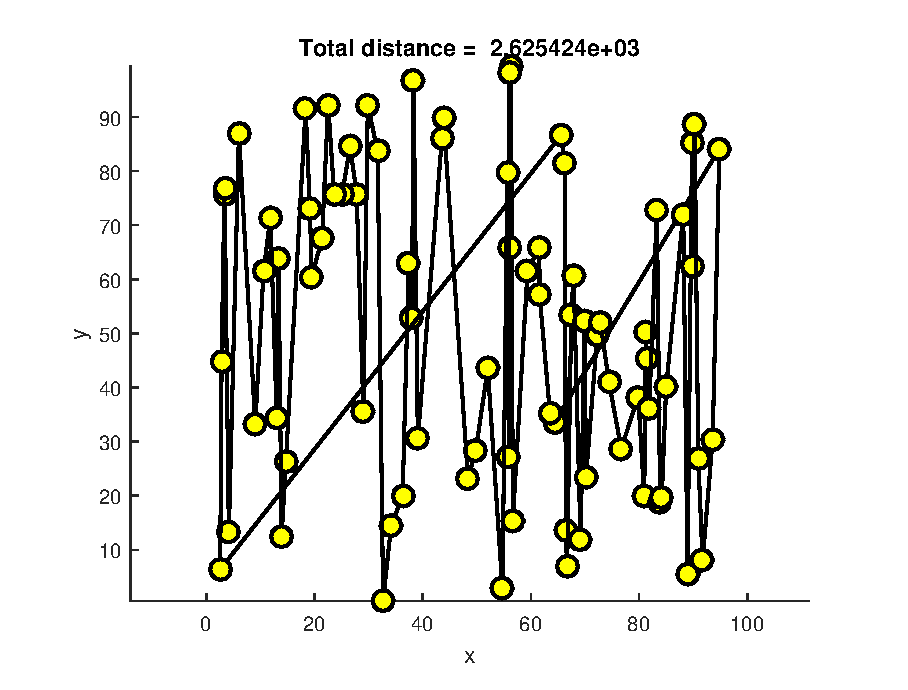
\includegraphics[width=\textwidth]{\Pathofhuit/path.eps}
		\caption{Path journey}\label{fig:Pathofhuit:path}
		
		\end{minipage}\hfill
		\begin{minipage}[t]{0.45\linewidth}
		\centering
		\includegraphics[width=\textwidth]{\Pathofhuit/AS_1_5AS_ExecTimeAndMeanSTDWith_execVariation.eps}
		\caption{Variation of the execution time VS the \# of ants (20$\stackrel{step=20}{\rightarrow}$100) in each execution (1$\stackrel{step=1}{\rightarrow}$ 5)}
		\label{fig:Pathofhuit:AS_1_5AS_ExecTimeAndMeanSTDWith_execVariation}
		\end{minipage}
	\flushleft
		\begin{minipage}[t]{0.45\linewidth}
		\centering
		\includegraphics[width=1.5\textwidth]{\Pathofhuit/AS_BestCost_Varying_Iteration_and_nbAnts.eps}
		\caption{Best cost VS Ants number variation with $\alpha$=1, $ \beta $ = 5}
		\label{fig:Pathofhuit:AS_BestCost_Varying_Iteration_and_nbAnts}
		\end{minipage}
	\end{figure}\flushright
		\begin{minipage}[t]{0.9\linewidth}
		\vspace{-9mm}
		\begin{table}[H]
		\label{tab:Pathofhuit:expdeux}
		\begin{tabular}{lllll}
		\cline{1-2}
		\multicolumn{1}{|l|}{Best Costs results for experience 2}                                                           &  \multicolumn{1}{l|}{Elapsed Time, Mean, STD}                                             &  &  &  \\ \cline{1-2}
		\multicolumn{1}{|l|}{\begin{tiny}\begin{tabular}{|l|c|c|c|c|c|c|c|c|c|c|}
\hline
&\textbf{It :1}&\textbf{It :2}&\textbf{It :3}&\textbf{It :4}&\textbf{It :5}&\textbf{It :6}&\textbf{It :7}&\textbf{It :8}&\textbf{It :9}&\textbf{It :10}\\\hline
\textbf{exec :1}&927.17&887.16&887.16&887.16&859.26&859.26&859.26&859.26&859.26&859.26\\\hline
\textbf{exec :2}&901.14&901.14&901.14&896.91&896.91&866.44&866.44&866.44&866.44&866.44\\\hline
\textbf{exec :3}&887.75&887.75&887.75&858.12&858.12&858.12&858.12&858.12&858.12&858.12\\\hline
\textbf{exec :4}&890.27&890.27&890.27&890.27&885.64&864.35&864.35&864.35&864.35&864.35\\\hline
\textbf{exec :5}&871.95&858.24&858.24&858.24&858.24&858.24&858.24&858.24&858.24&844.82\\\hline
\textbf{exec :6}&814.81&814.81&814.81&814.81&814.81&814.81&814.81&814.81&814.81&814.81\\\hline
\textbf{exec :7}&869.78&863.12&863.12&845.72&845.72&837.21&837.21&837.21&837.21&837.21\\\hline
\textbf{exec :8}&873.76&840.97&799.51&799.51&799.51&799.51&799.51&799.51&799.51&799.51\\\hline
\textbf{exec :9}&868.26&817.51&817.51&817.51&817.51&817.51&817.51&817.51&817.51&814.99\\\hline
\textbf{exec :10}&842.73&835.77&812.00&812.00&812.00&812.00&812.00&812.00&812.00&812.00\\\hline
\end{tabular}
\end{tiny}} & \multicolumn{1}{l|}{\begin{tiny}\begin{tabular}{|l|c|}
\hline
&\textbf{Elapsed time}\\\hline
\textbf{exec :1}&3.20\\\hline
\textbf{exec :2}&3.22\\\hline
\textbf{exec :3}&3.20\\\hline
\textbf{exec :4}&3.21\\\hline
\textbf{exec :5}&3.22\\\hline
\textbf{exec :6}&3.21\\\hline
\textbf{exec :7}&3.21\\\hline
\textbf{exec :8}&3.21\\\hline
\textbf{exec :9}&3.23\\\hline
\textbf{exec :10}&3.21\\\hline
\textbf{ Mean}&3.21\\\hline
\textbf{ STD}&0.01\\\hline
\end{tabular}
\end{tiny} } &  &  &  \\ \cline{1-2}
																						  &                                                                     &  &  &  \\
																						  &                                                                     &  &  & 
		\end{tabular}
		\caption{Results of experience 2 on rand80.dat}
		\end{table}
		\end{minipage}	

%%\end{figure}